\section{Solutions on the Market}
%Meta + Short descript of the ones chosen solutions(the intro in knowledge sec)
The solutions in question are the five following:
\begin{itemize}
    \item Fleet Management Software 4.0
    \item TomTom Webfleet
    \item Teletrac Navman Director
    \item Geotab
    \item Fleetio
\end{itemize}
Each of the different fleet management systems allow for either manual or automatic tracking of the daily use of the different vehicles and we will group them as such when taking a closer look.
%Most of the systems also allow for tracking of the vehicles through GPS and advanced vehicle information, such as price per kilometre and driving behaviors.

\begin{figure}[h!]
    \centering
    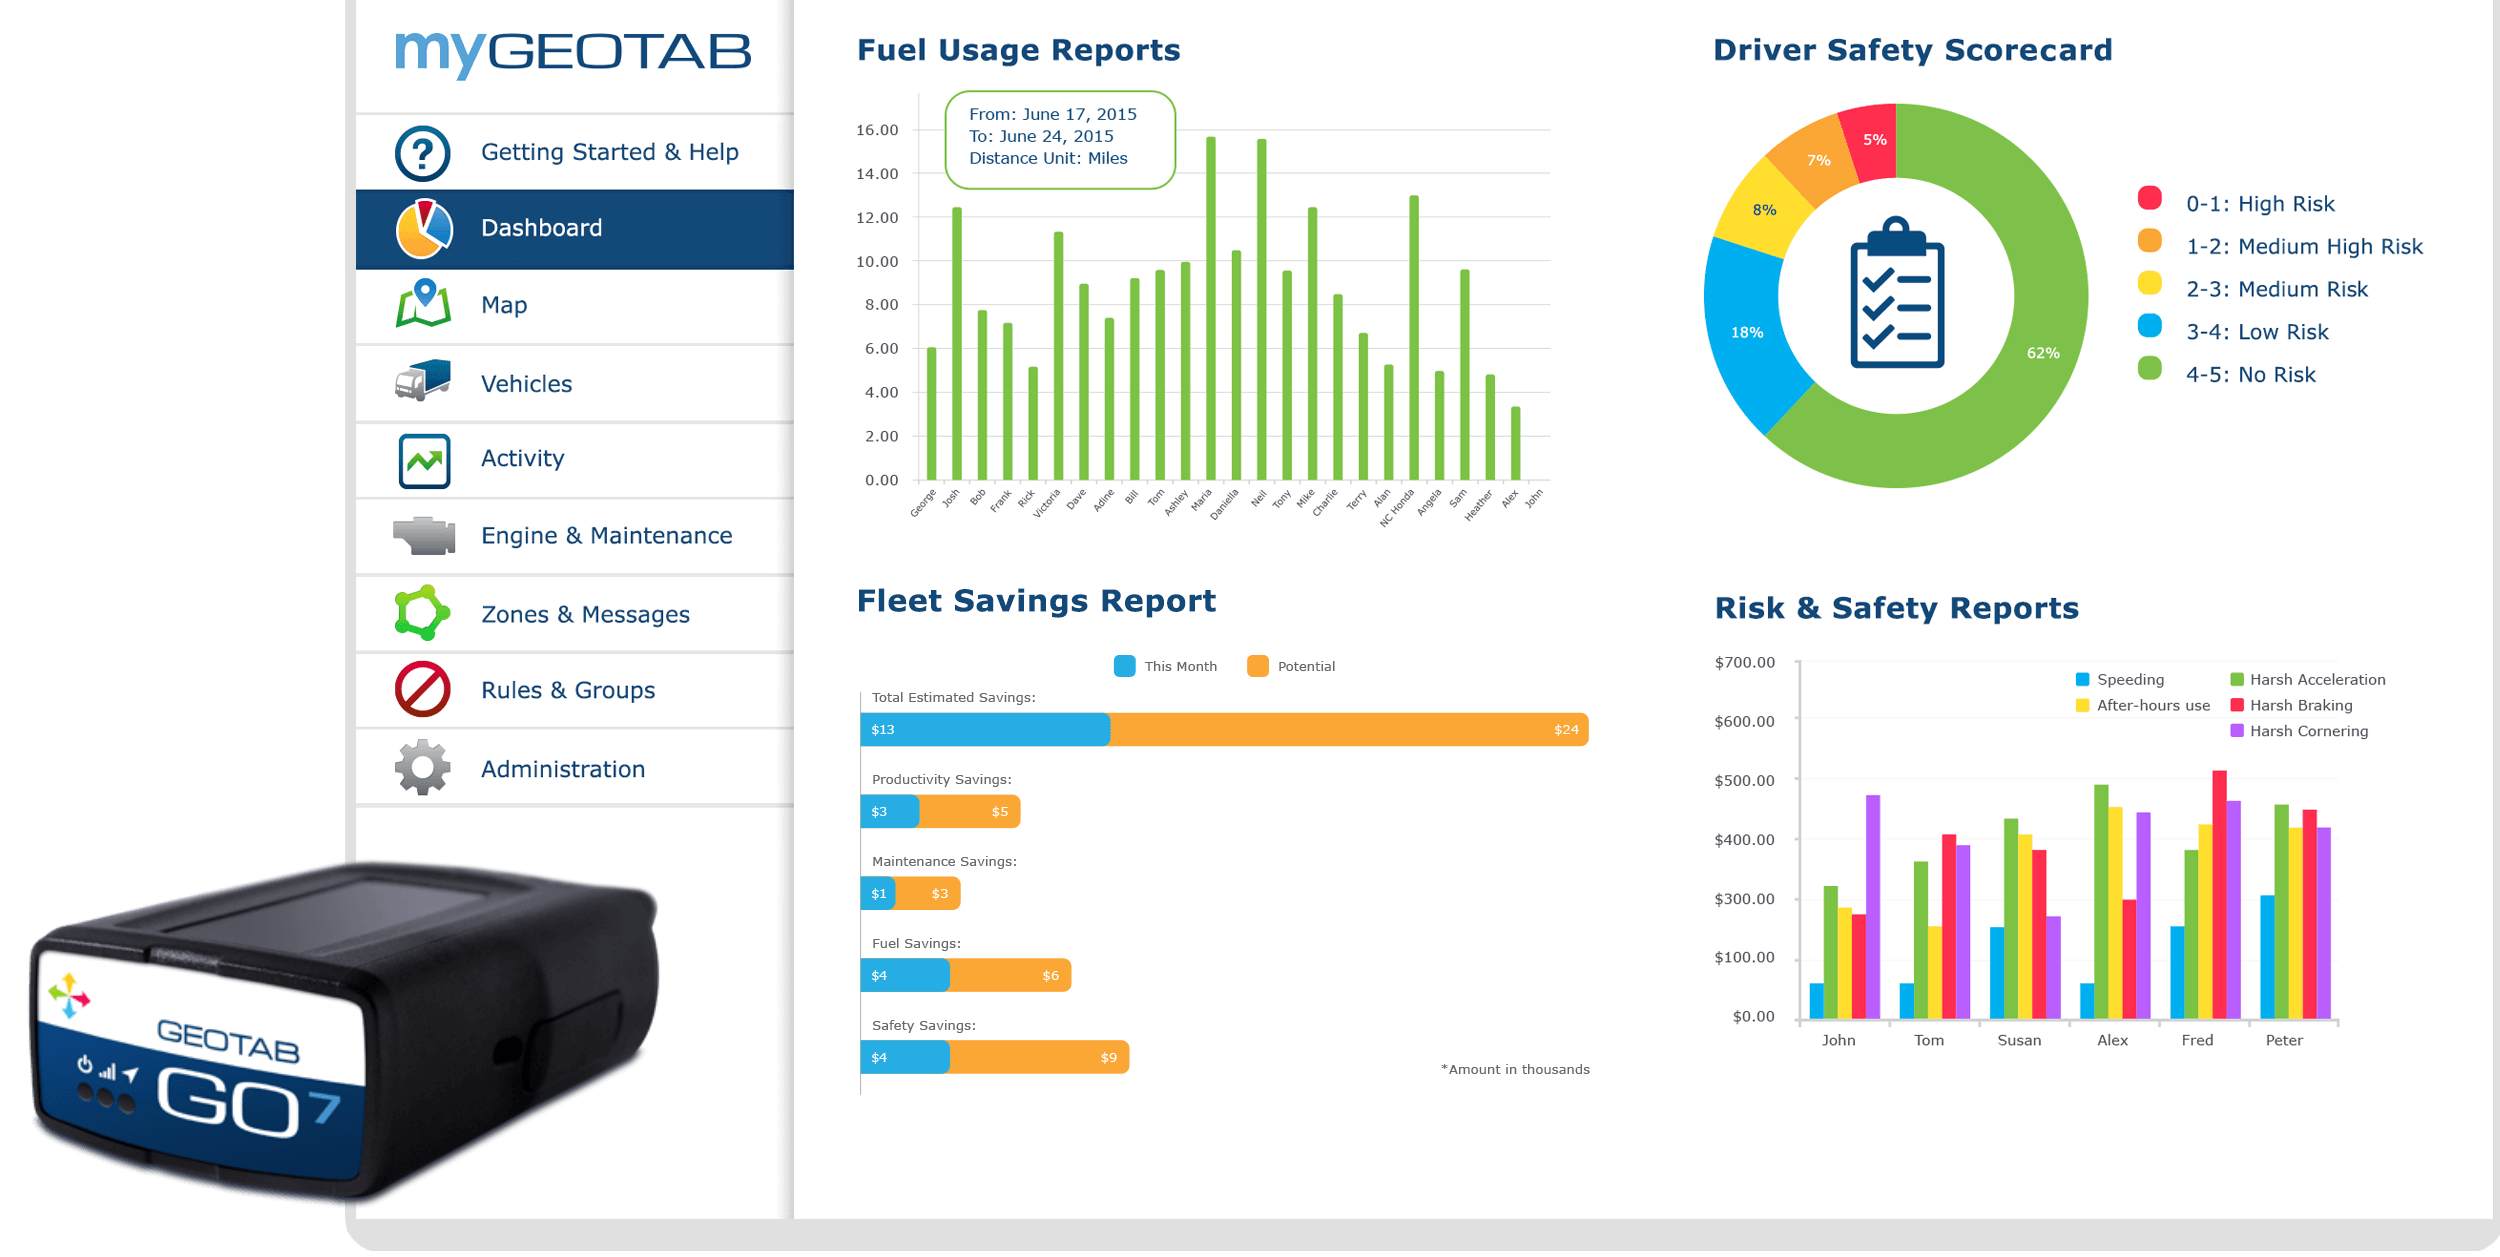
\includegraphics[width=0.5\textwidth]{img/Geotab_device_dashboard.png}
    \caption{Display of the TomTomlink, and TomTom Geotab Dashboard.}
    \label{fig:TomTom_TomTomlink_GeotabDashboard}
\end{figure}

\subsection{Manual Data Collection}

\begin{figure}[h!]
    \centering
    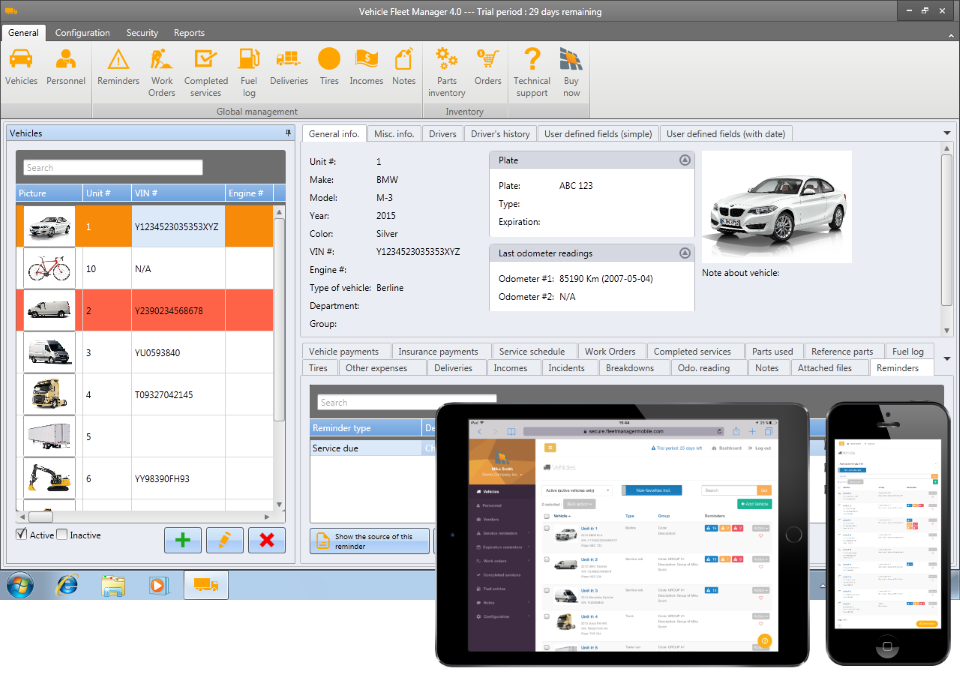
\includegraphics[width=0.5\textwidth]{img/FleetManagementSoftware.png}
    \caption{Dashboard and mobile application for Fleet Management Software 4.0.}
    \label{fig:Fleet_Management_Software}
\end{figure}
\textit{Fleet Management Software 4.0} is the only of the chosen solutions that uses strictly manual data collection.
The downside to this is that everything is handled by the drivers, as such manual systems are essentially just data analysis systems.
Fleet Management Software 4.0 does not have any recurring payments, it consists of a single time fee of \$90.
This makes it have the highest initial cost, unlike the other solutions Fleet Management Software 4.0 does not get any more expensive over time.

\subsubsection{Fleet Management Software 4.0}
%%%%%
%From Knowledge
\textit{Fleet Management Software 4.0} is developed by Vinity Soft, and focuses on keeping track of vehicle expenses, creating maintenance programs and service schedules\cite{vinitysoft}.
%From understanding
This solution uses manual tracking, and allows the user to store documents with information pertaining the different vehicles in the fleet.
Some of the other tools which are available through \textit{Fleet Management Software 4.0} includes scheduling vehicles for maintenance and a limited way of calculating the expense of the drivers.
As mentioned this is a manual system, as such all information is provided by the user when an action is performed, such as refueling.
%%%%%
\subsection{Automatic Data Collection}%These secs will rely on info from the understanding and the expanded section from knowledge sec going into a little more detail for each
\begin{figure}[h!]
    \centering
    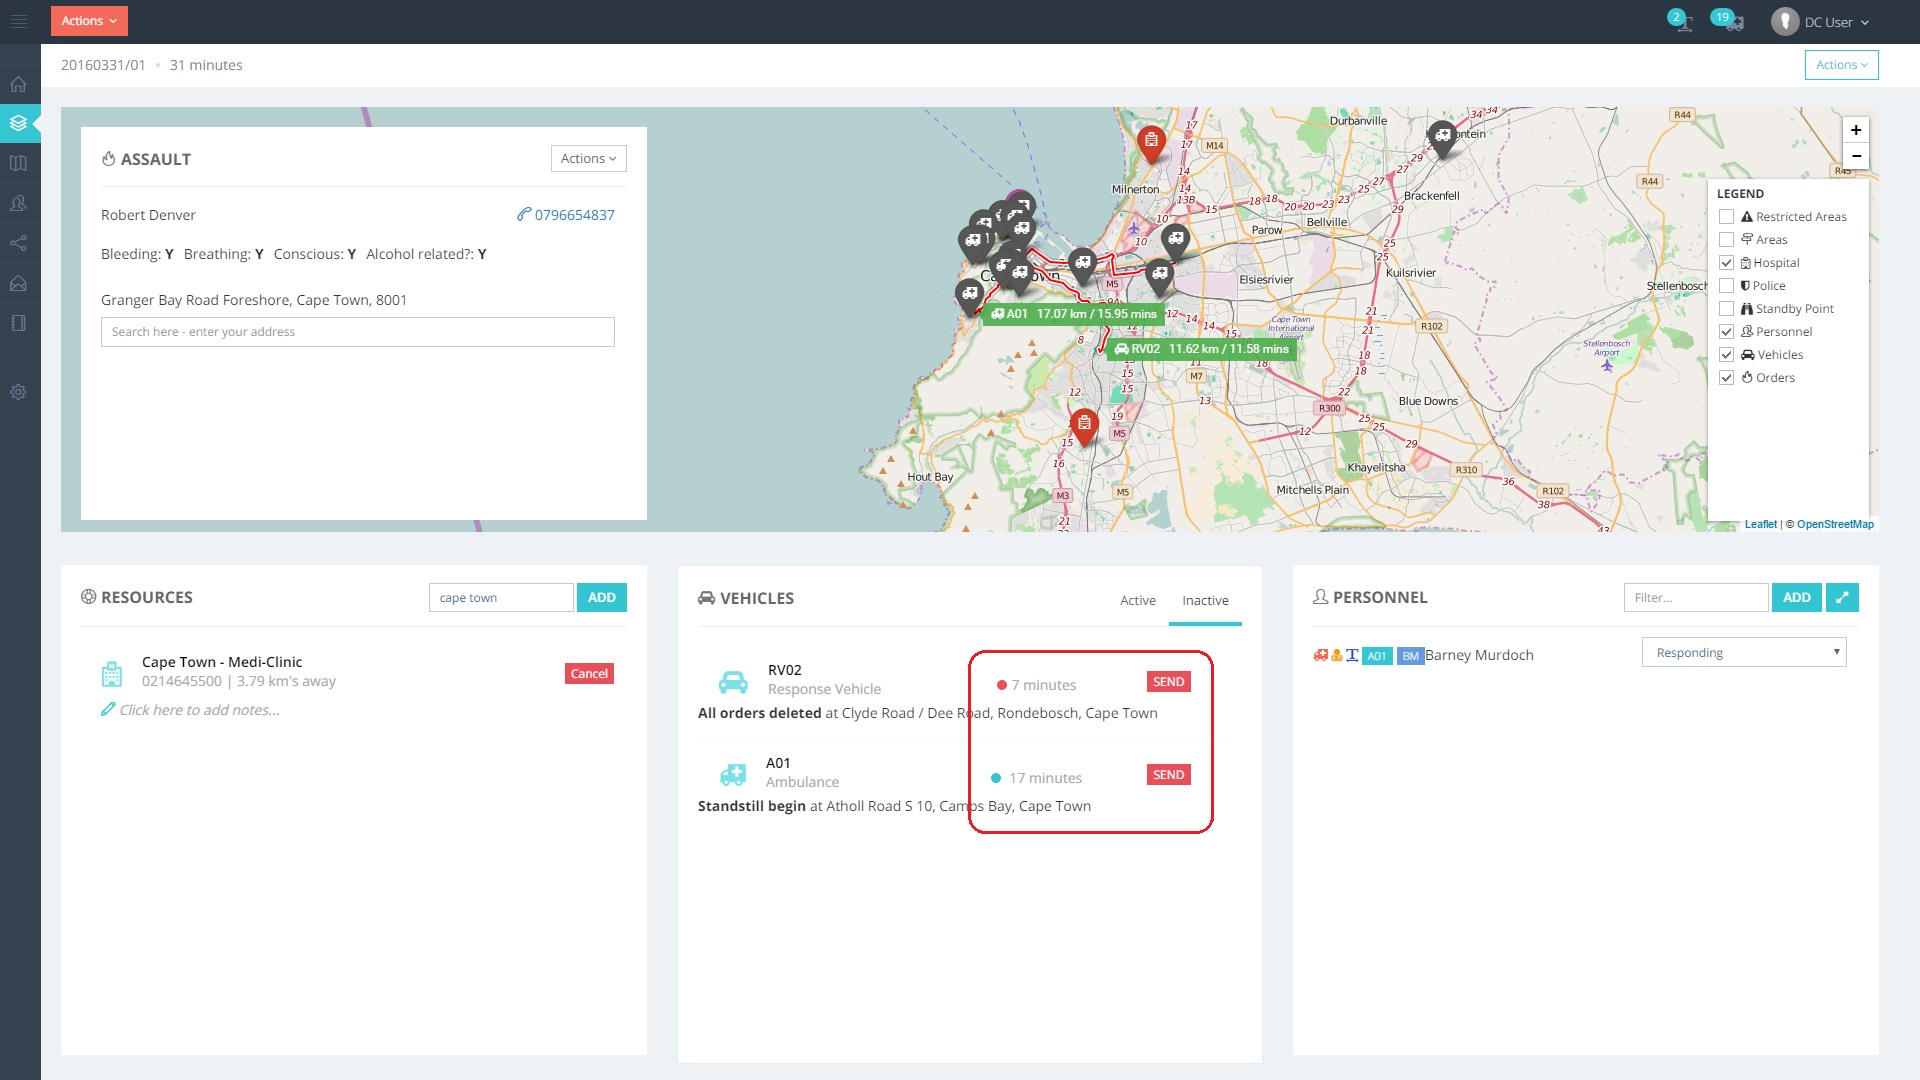
\includegraphics[width=0.5\textwidth]{img/tomtom_webfleet.jpeg}
    \caption{Illustration of the TomTom Webfleet dashboard.}
    \label{fig:TomTom_Webfleet}
\end{figure}
\textit{TomTom Webfleet}, \textit{Teletrac Navman Director} and \textit{Geotab} are all fully automatic systems where the driver provides no input, as such the system simply needs to be installed to work.
As for prices they the monthly cost for the \textit{TomTom} solution ranges from \$16 to \$25 per month per vehicle\footnote{Price range for TomTom Webfleet\\ \url{https://telematics.tomtom.com/en_gb/webfleet/fleet-management/vehicle-tracking/entry-level/}}.
There are two price levels; \$16 limiting the vehicle to the UK and \$25 for tracking beyond UK borders which is still limited to only the majority of european countries.
The solution from \textit{GeoTab} costs around \$24 per month per vehicle, however this solution also requires the OBD device which costs \$99 per vehicle\footnote{GeoTab Price \url{http://www.anythinggps.com/index.php?route=product/product\&product_id=51}}.
Teletrac is a subscription based service\footnote{Teletrac Navman Director pricing model\url{https://www.getapp.com/operations-management-software/a/teletrac/\#pricing}}, however Teletrac does not directly offer any prices, a company must contact Teletrac in order to get a price estimate.

\subsubsection{TomTom Webfleet \& Teletrac Navman Director}
\begin{figure}[h!]
    \centering
    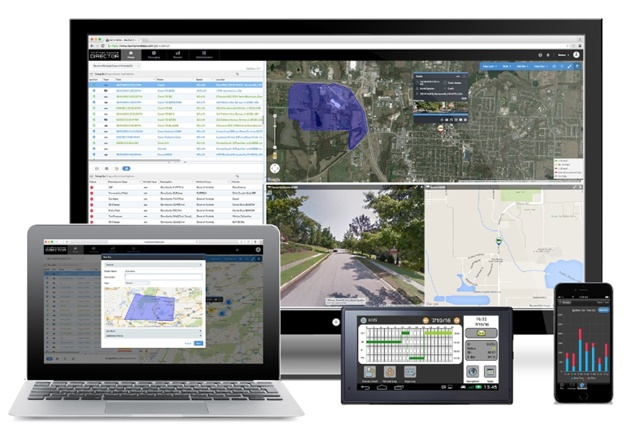
\includegraphics[width=0.5\textwidth]{img/TELETRAC.jpg}
    \caption{Dashboard and mobile application for Teletrac Navman Director.}
    \label{fig:TELETRAC_NAVMAN_DIRECTOR}
\end{figure}
\textit{TomTom Webfleet} and \textit{Teletrac Navman Director} both focus on the driver aspects in fleet management, as such they also have quite a few similarities.
Some of these similarities are:
\begin{description}
    \item Overview of driving behaviour.
    \item Calculating the expenses for each of the drivers.
    \item Live overview of the fleet via GPS.
    \item Keeping track of the delivery time.
\end{description}
%%%%%
As for their dissimilarities \textit{TomTom Webfleet} is developed by the Dutch company TomTom which is known for their GPS navigation systems. This solution uses the TomTom LINK device to track vehicles' position and movement, and transmits this information to the \textit{Webfleet} dashboard. TomTom also provide an API for integration with existing systems \cite{tomtom}.
\textit{Teletrac Navman Director} provides tools for fleet and asset management, driver behaviour, and safety \cite{teletracnavman}.
Teletrac uses an electronic logging device, which is mounted in each car to receive its information\footnote{The Cost of Compliance: An ELD Price Comparison \url{http://www.teletracnavman.com/blog/us/eld_price_comparison.pdf}}.
%From understanding
%%%%%
\subsubsection{Geotab}
%%%%%
%From Knowledge

\textit{Geotab}'s solution uses a device, which can be seen in \cref{fig:Geotab_device}, which is to be mounted in the vehicles in order to track them. MyGeotab, which is the online dashboard for \textit{Geotab}, is able to track the position of the different vehicles it is also able to detect vehicle accidents\cite{geotab}.
\begin{figure}[h!]
    \centering
    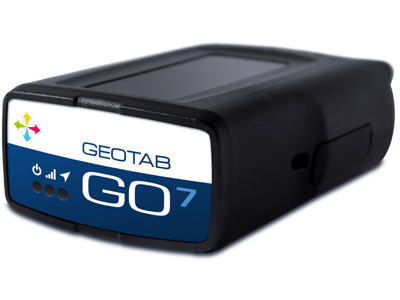
\includegraphics[width=0.5\textwidth]{img/geotab-device-side-view.png}
    \caption{Geotab's uses a Plug-\&-Play OBD--II device}
    \label{fig:Geotab_device}
\end{figure}

\textit{Geotab} also allow for maintenance reminders triggered by a time interval or distance driven.
%From understanding
\textit{Geotab} uses a Plug-\&-Play OBD--II device which has to be mounted into each of the vehicles, the device then transmit all the data to \textit{Geotab}'s system.
This allows \textit{Geotab} to gather live engine information, this information is then interpreted and analysed according to some criteria established by \textit{Geotab} which the system uses to detect vehicle accidents remotely\footnote{Geotab remote accident tracking \url{https://docs.google.com/document/d/1rOJZzzZhoKXWrmswaseUr3Wk8h_nPXPK4yFtdi6yVJ0/edit}}, however these specific criteria is not available to the public.
%%%%%
\subsection{Hybrid Data Collection}
Whereas all the previous solutions were either fully automatic or fully manual, \textit{Fleetio} allows for both manual and automatic data collection allowing for a broader range of data.
Comparitively \textit{Fleetio} is also the cheapest choice by far.
\textit{Fleetio} has two different packages to choose between, the pro plan at \$3 per month per vehicle and the advanced plan at \$5 per month per vehicle\footnote{Pricing for Fleetio \url{https://www.fleetio.com/pricing}}.
\subsubsection{Fleetio}
%%%%%
%From Knowledge
\textit{Fleetio}'s solution takes advantage of the driver's phone, instead of requiring a separate device for data gathering.
\textit{Fleetio} focuses on managing vehicle data, keeping track of fleet maintenance and increasing the effectiveness of a company \cite{fleetio}.
%From understanding
In the scenarios where the system was fully automated, the solutions required the company to invest in devices which should be mounted in each vehicle.
This is done in order for the solutions to gather the necessary information.
In the exact opposite case where the solution were completely manual this would require the company to invest a noticeable amount of time into the system in order for it to be up to date.

In order for \textit{Fleetio} to automate as much as possible, \textit{Fleetio} utilises the phone of the driver to track the current position, speed of the vehicle and estimated fuel consumption.

For information such as calculating the expense of each of the drives by manually inputting the cost after refuelling each vehicle.
\textit{Fleetio} is cheaper than the other solutions we have looked at, easy to install alternative to bigger and more extensive fleet management systems, which already exists.
\textit{Fleetio} has managed to locate a gap in the market, this gap being the use of pre--existing hardware, e.g. the drivers phone.
This helps maintaining a low initial cost since no new hardware is required.
If a company decides to change from another company such as either \textit{TomTom} or \textit{Geotab}, \textit{Fleetio} is compatible with with the hardware those solutions require.
%%%%%
%%%%%
